% Options for packages loaded elsewhere
\PassOptionsToPackage{unicode}{hyperref}
\PassOptionsToPackage{hyphens}{url}
%
\documentclass[
  letterpaperpaper,
]{article}
\usepackage{lmodern}
\usepackage{amssymb,amsmath}
\usepackage{ifxetex,ifluatex}
\ifnum 0\ifxetex 1\fi\ifluatex 1\fi=0 % if pdftex
  \usepackage[T1]{fontenc}
  \usepackage[utf8]{inputenc}
  \usepackage{textcomp} % provide euro and other symbols
\else % if luatex or xetex
  \usepackage{unicode-math}
  \defaultfontfeatures{Scale=MatchLowercase}
  \defaultfontfeatures[\rmfamily]{Ligatures=TeX,Scale=1}
\fi
% Use upquote if available, for straight quotes in verbatim environments
\IfFileExists{upquote.sty}{\usepackage{upquote}}{}
\IfFileExists{microtype.sty}{% use microtype if available
  \usepackage[]{microtype}
  \UseMicrotypeSet[protrusion]{basicmath} % disable protrusion for tt fonts
}{}
\makeatletter
\@ifundefined{KOMAClassName}{% if non-KOMA class
  \IfFileExists{parskip.sty}{%
    \usepackage{parskip}
  }{% else
    \setlength{\parindent}{0pt}
    \setlength{\parskip}{6pt plus 2pt minus 1pt}}
}{% if KOMA class
  \KOMAoptions{parskip=half}}
\makeatother
\usepackage{xcolor}
\IfFileExists{xurl.sty}{\usepackage{xurl}}{} % add URL line breaks if available
\IfFileExists{bookmark.sty}{\usepackage{bookmark}}{\usepackage{hyperref}}
\hypersetup{
  pdftitle={Homework 1 (Due September 6th)},
  hidelinks,
  pdfcreator={LaTeX via pandoc}}
\urlstyle{same} % disable monospaced font for URLs
\usepackage{longtable,booktabs}
% Correct order of tables after \paragraph or \subparagraph
\usepackage{etoolbox}
\makeatletter
\patchcmd\longtable{\par}{\if@noskipsec\mbox{}\fi\par}{}{}
\makeatother
% Allow footnotes in longtable head/foot
\IfFileExists{footnotehyper.sty}{\usepackage{footnotehyper}}{\usepackage{footnote}}
\makesavenoteenv{longtable}
\usepackage{graphicx,grffile}
\makeatletter
\def\maxwidth{\ifdim\Gin@nat@width>\linewidth\linewidth\else\Gin@nat@width\fi}
\def\maxheight{\ifdim\Gin@nat@height>\textheight\textheight\else\Gin@nat@height\fi}
\makeatother
% Scale images if necessary, so that they will not overflow the page
% margins by default, and it is still possible to overwrite the defaults
% using explicit options in \includegraphics[width, height, ...]{}
\setkeys{Gin}{width=\maxwidth,height=\maxheight,keepaspectratio}
% Set default figure placement to htbp
\makeatletter
\def\fps@figure{htbp}
\makeatother
\setlength{\emergencystretch}{3em} % prevent overfull lines
\providecommand{\tightlist}{%
  \setlength{\itemsep}{0pt}\setlength{\parskip}{0pt}}
\setcounter{secnumdepth}{-\maxdimen} % remove section numbering

\title{Homework 1 (Due September 6th)}
\date{}

\begin{document}
\maketitle

\href{http://msuphysics481fall2019.slack.com}{\textbf{Link to Slack
team}}

\hypertarget{preface}{%
\subsubsection{Preface}\label{preface}}

Homework in this class is a very large part of the learning experience
(and a large fraction of your grade!). The homework might look long, but
that is because it is not really serving as a check on whether you are
getting things from lecture. It is meant to help you learn the material,
the importance of different aspects of the material, and the
implications of the material on your future work. So there will
typically be longer descriptions in the problem statements. The work you
are being asked to do is no longer than a standard lecture course, but
the kinds of questions might be different. We strongly encourage you to
work together (and with the Bryan and Danny) on these homework problems,
but you must turn in your own work.

\hypertarget{submitting-your-homework}{%
\subsubsection{Submitting your
homework}\label{submitting-your-homework}}

All of your pencil-and-paper solutions can be turned in at the beginning
of class on Friday. Homework solutions that require Python are to be
turned in online using Dropbox file requests. Each homework assignment
will have a different file request link. Make sure that your name
appears in the filename of the notebook (e.g.,
notebook\_for\_problem\_4\_dannycaballero.ipynb). For homeworks with
multiple notebook submissions, you may either combine the notebooks or
submit separate notebooks for each problem.

\hypertarget{what-is-homework-1-about}{%
\subsubsection{What is Homework 1
about?}\label{what-is-homework-1-about}}

Homework 1 emphasizes the mathematical formalism and related thinking
that you will draw on in this class. This homework focuses on Sections
1.1-1.4 of Griffiths, which covers differential, integral, and vector
calculus. It also serves as an introduction to using
\href{http://jupyter.org}{Jupyter notebooks}, which you will use on most
homework assignments. With regard to computation on this homework, you
will be using the \href{http://matplotlib.org/}{matplotlib} library,
which allows you to plot different kinds of figures. These first few
computational exercises will serve as an introduction to (or a reminder
of) the kinds of things we will do with Python this semester.

\hypertarget{link-for-code-submissions}{%
\subsubsection{Link for code
submissions}\label{link-for-code-submissions}}

\href{https://www.dropbox.com/request/TWSUUsUgJ7zKmQeAuDzB}{\textbf{Dropbox
file request link for Homework 1}}

\hypertarget{homework-questions}{%
\subsubsection{Homework questions}\label{homework-questions}}

\hypertarget{reminders-of-integrals-past}{%
\paragraph{1. Reminders of Integrals
Past}\label{reminders-of-integrals-past}}

In this course, you will perform lots of different kinds of integrals,
some of which you might have done in previous courses. In this problem,
we will just dust off some of those integration techniques. To earn full
credit, you will need to explain key steps of the integration for each
one, not simply do the mathematics.

\begin{enumerate}
\def\labelenumi{\arabic{enumi}.}
\tightlist
\item
  \emph{Line (or path) integrals} - These integrals are important for
  thinking about energy (and in our case electric potential).
\end{enumerate}

\begin{itemize}
\tightlist
\item
  Determine the work done by the vector force
  \(\mathbf{F} = y^2\;\hat{x} - 2x^2\;\hat{y}\) along the path \(y=x^2\)
  from (0,0) to (3,9). This path is restricted to the x-y plane and
  recall that \(W=\int \mathbf{F}\cdot d\mathbf{l}\).
\item
  Is the result of this line integral path-independent (i.e., is
  \(\mathbf{F}\) a
  \href{https://en.wikipedia.org/wiki/Conservative_vector_field}{conservative
  vector field})? Explain why or why not.
\end{itemize}

\begin{enumerate}
\def\labelenumi{\arabic{enumi}.}
\setcounter{enumi}{1}
\tightlist
\item
  \emph{Surface integrals} - Calculating the flux over a particular
  surface is a very common way of determine the electric field.
\end{enumerate}

\begin{itemize}
\tightlist
\item
  Evaluate the integral \(\int_S \mathbf{v}\cdot d\mathbf{A}\) where
  \(\mathbf{v}(x,y,z) = 5x\;\hat{y} + 2y\;\hat{z}\) and \(S\) is the
  rectangular surface lying in x-z plane from (0,0,0) to (1,0,5). Choose
  the direction of \(+\hat{y}\) to be indicative of positive flux.
\item
  Explain how the resulting sign of the flux makes sense. You may use
  sketches or diagrams.
\end{itemize}

\begin{enumerate}
\def\labelenumi{\arabic{enumi}.}
\setcounter{enumi}{2}
\tightlist
\item
  \emph{Volume integrals} - It will be common for you to determine the
  amount of total charge in a situation where the charge is distributed
  in space according to some function. You might be familiar with this
  concept from the perspective of distributed mass in Classical
  Mechanics.
\end{enumerate}

\begin{itemize}
\tightlist
\item
  Consider two different spheres: one with uniform mass density,
  \(\rho_0\), and the other with a radially varying density,
  \(\rho(r)=\frac{3\rho_0}{4R^2}r^2\).
\item
  If both spheres have the same radius \(R\), which has more mass?
\end{itemize}

\hypertarget{what-operations-can-be-done-to-different-kinds-of-functions}{%
\paragraph{2. What operations can be done to different kinds of
functions?}\label{what-operations-can-be-done-to-different-kinds-of-functions}}

\begin{enumerate}
\def\labelenumi{\arabic{enumi}.}
\tightlist
\item
  Given the scalar function \(T(x,y,z)\) (e.g., the temperature at any
  point in the room), which of the three operations (div, grad, and/or
  curl) can be sensibly operated on \(T\)? For each which can:
\end{enumerate}

\begin{itemize}
\tightlist
\item
  give a formula for the result,
\item
  explain in words how you would interpret the result, and
\item
  identify if the result a vector or scalar.
\end{itemize}

\begin{enumerate}
\def\labelenumi{\arabic{enumi}.}
\setcounter{enumi}{1}
\tightlist
\item
  Given the vector function \(\vec{V}(x,y,z)\) (e.g., the velocity of a
  flowing fluid), which of the three operations (div, grad, and/or curl)
  can be sensibly operated on \(\vec{V}\)? For each which can:
\end{enumerate}

\begin{itemize}
\tightlist
\item
  give a formula for the result,
\item
  explain in words how you would interpret the result, and
\item
  identify if the result a vector or scalar.
\end{itemize}

\hypertarget{determine-the-gradient-of-a-scalar-function}{%
\paragraph{3. Determine the gradient of a scalar
function}\label{determine-the-gradient-of-a-scalar-function}}

In Griffiths, \(\vec{\mathfrak{r}}\) represents the separation vector
between source charges \(\langle x', y', z' \rangle\) and the field
point -- location of test charge -- \(\langle x, y, z \rangle\). The
separation vector is a \textbf{critically important} vector in
electrodynamics as it underlies all of the mathematical models that
describe how source charges produce electric and magnetic fields. To
that end, you will often do some mathematical manipulations of the
separation vector. You are asked to perform two common manipulations
below.

\begin{enumerate}
\def\labelenumi{\arabic{enumi}.}
\tightlist
\item
  Calculate the gradient of the magnitude of the separation vector
  (i.e., \(\nabla\|\vec{\mathfrak{r}}\|\)).
\item
  Calculate the gradient of the inverse of the magnitude of the
  separation vector (i.e.,
  \(\nabla \dfrac{1}{\|\vec{\mathfrak{r}}\|}\)).
\item
  Show the gradients of these functions can be written as functions of
  the separation vector (\(\vec{\mathfrak{r}}\)) and/or its magntiude
  (\(\|\vec{\mathfrak{r}}\|\)). (\emph{Hint: it might be easier to do
  this by explicitly writing out the function in Cartesian
  coordinates.})
\item
  What vector identities have you developed for the separation vector?
  This is just asking you to state them based on your answers from parts
  1, 2, and 3.
\end{enumerate}

\hypertarget{analyzing-divergence-and-curl-visually}{%
\paragraph{4. Analyzing divergence and curl
visually}\label{analyzing-divergence-and-curl-visually}}

Calculating the divergence and curl of a vector field analytically is
possible when the field is a well-known function (e.g.,
\(\vec{V}(x,y,z)\)). However, it will not always be the case that you
know the function that generates the vector field. For example, in
experimental fluid mechanics, measurements of the velocity field are
done by tracking individual particles (called ``tracers'') that move in
the field.

\href{https://www.youtube.com/watch?v=hzvFHrWQbP0}{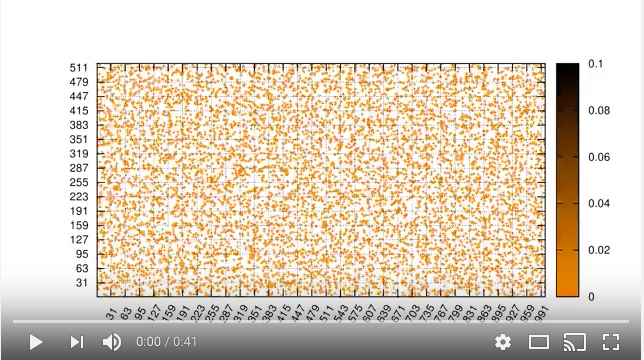
\includegraphics{./images/hw1/tracers.png}}

The displacement of those tracers is used to numerically reconstruct the
velocity field of the fluid (by way of numerical derivatives), which
usually does not conform to a known function. However, it is important
to know if the flow has divergence or curl overall or at specific points
as the models for fluid flow that are used to analyze the velocity field
strongly depend on these results. Hence, visual inspection of a field
(in our case, electromagnetic fields) is an important tool to understand
which models might be used to analyze the field. This will be
exceedingly important in our distinction between electric and magnetic
fields as well as when the fields begin to vary with time.

For each of the four vector fields sketched below:

\begin{enumerate}
\def\labelenumi{\arabic{enumi}.}
\tightlist
\item
  Which of them have a nonzero \emph{divergence} somewhere? (If the
  divergence is nonzero \emph{only} at isolated points, which point(s)
  would that be?)
\item
  Which of the following fields have nonzero \emph{curl} somewhere? (If
  the curl is nonzero \emph{only} at isolated points, which point(s)
  would that be?)
\item
  Provide a brief explanation for each of your answers above.
\end{enumerate}

\begin{longtable}[]{@{}cc@{}}
\toprule
\endhead
Field A & Field B\tabularnewline
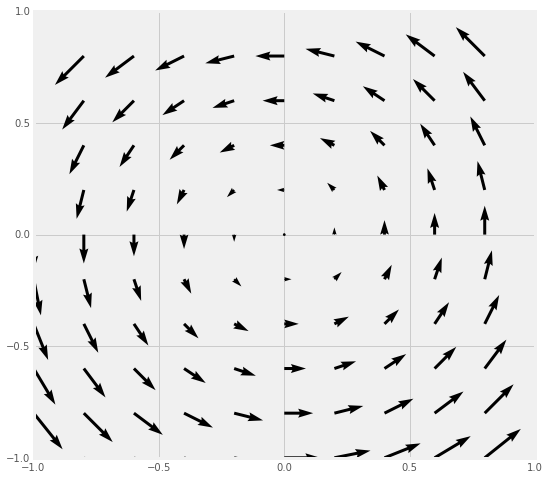
\includegraphics{./images/hw1/A.png} &
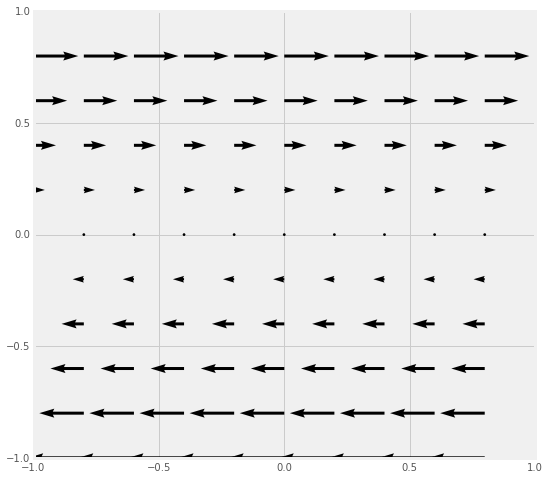
\includegraphics{./images/hw1/B.png}\tabularnewline
Field C & Field D\tabularnewline
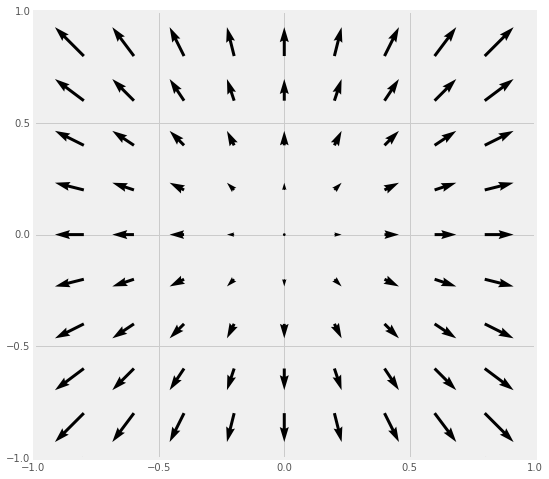
\includegraphics{./images/hw1/C.png} &
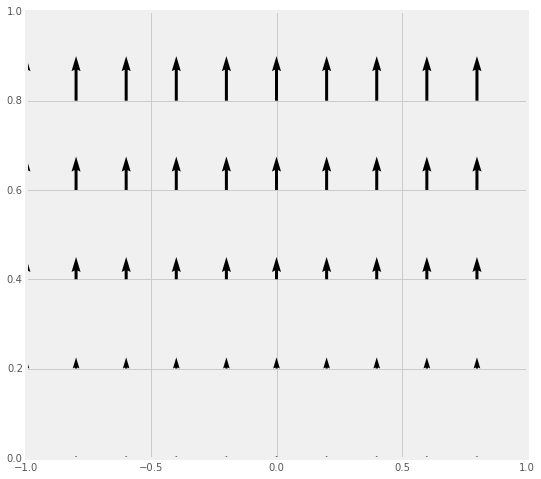
\includegraphics{./images/hw1/D.png}\tabularnewline
\bottomrule
\end{longtable}

\hypertarget{plotting-vector-functions-with-matplotlib}{%
\paragraph{\texorpdfstring{5. Plotting vector functions with
\texttt{matplotlib}}{5. Plotting vector functions with matplotlib}}\label{plotting-vector-functions-with-matplotlib}}

Physics is both a mathematical and visual science. It is important to
develop the ability to sketch and plot figures of various types. For the
early part of this class, plotting the field generated by electric
charges is important to understanding the field itself. In this problem,
you will learn to use the
\href{http://matplotlib.org}{\texttt{matplotlib} library} to
\href{http://matplotlib.org/examples/pylab_examples/quiver_demo.html}{plot
vector fields}. As with the previous computational problem, you can
\href{../jupyter/HW1-VectorFieldsProblem.ipynb}{download this working
Jupyter notebook}
(\href{https://github.com/dannycab/phy481msu_f2019/blob/master/jupyter/HW1-VectorFieldsProblem.ipynb}{view
it here}), which describes how this kind of plotting is done for a
specific case (\(\vec{v}(x,y)=y\hat{x}\)).

It will be up to you to plot additional figures for these cases:

\begin{enumerate}
\def\labelenumi{\arabic{enumi}.}
\tightlist
\item
  \(\vec{v}(x,y)=r\hat{r}\) (where \(\vec{r}\) refers to the usual
  \(\vec{r}\) in spherical coordinates.)
\item
  \(\vec{v}(x,y)=\hat{r}/r\)
\item
  \(\vec{v}(x,y) = \dfrac{x}{(\sqrt{x^2+y^2})^3}\hat{x}+\dfrac{y}{(\sqrt{x^2+y^2})^3}\hat{y}\)
\item
  \(\vec{v}(x,y) = \hat{\phi}\) (where \(\\phi\) is the usual
  plane-polar coordinate.)
\item
  For each case above, can you describe a physical situation where the
  field would be applicable?
\end{enumerate}

\textbf{When we construct different kinds of fields in this class, you
will use code like this to visualize the field and discuss it.}

You will turn in all parts of this problem via
\href{https://www.dropbox.com/request/TWSUUsUgJ7zKmQeAuDzB}{Dropbox file
request.}

\hypertarget{vector-proofs-can-be-incredibly-useful}{%
\paragraph{6. Vector proofs can be incredibly
useful}\label{vector-proofs-can-be-incredibly-useful}}

In electromagnetism, developing a deep understanding of vector
mathematics can facilitate a deeper understanding of the physical
systems that we will investigate. While we will rarely ask you to prove
relationships outright, knowing how certain proofs are done can often
help you simplify a complicated problem.

For example, in this problem, you will learn how we often use general
vector operations with unspecified surfaces to make general statements
about the field. In Griffiths, you read about a few integral theorems:
the gradient theorem, Gauss's theorem (for divergences), and Stokes'
theorem (for curls). You will make use of those theorems to prove a few
things to develop some intuition about vector calculus.

\begin{enumerate}
\def\labelenumi{\arabic{enumi}.}
\tightlist
\item
  From vector calculus, you know that the curl of any gradient of any
  scalar field is zero: $\nabla \times \nabla T(x,y,z) = 0 $.
\end{enumerate}

\begin{itemize}
\tightlist
\item
  Use the corollary of the gradient theorem, namely that closed loop
  integral of any gradient of a scalar field is zero,
  \(\oint \nabla T\cdot d\mathbf{l} = 0\), along with Stokes' theorem,
  \(\int_S(\nabla \times \mathbf{v})\cdot d\mathbf{a} = \oint_C \mathbf{v}\cdot d\mathbf{l}\),
  to demonstrate that the curl of a gradient is zero.
\item
  What is the essential argument that needs to be made that proves that
  the result is generalizable to any situation? (\emph{Hint: The surface
  (S) and thus the line (C) that bounds the surface are not specified.})
\item
  What does your result from the previous question tell you about
  possibility of swirly-ness of the gradient of a temperature field,
  \(\nabla T\), over any specified surface?
\end{itemize}

\begin{enumerate}
\def\labelenumi{\arabic{enumi}.}
\setcounter{enumi}{1}
\tightlist
\item
  From vector calculus, you know that the divergence of the curl of any
  vector field is zero, \(\nabla \cdot (\nabla \times \mathbf{v}) = 0\).
\end{enumerate}

\begin{itemize}
\tightlist
\item
  Use the corollary of Stokes' theorem, namely that the closed surface
  integral of the curl of a vector field is zero, $\oint\_S
  (\nabla \times \mathbf{v})\cdot d\mathbf{a} = 0 $, along with the
  divergence theorem,
  \(\int(\nabla \cdot \mathbf{v}) d\tau = \oint_S \mathbf{v}\cdot d\mathbf{a}\),
  to demonstrate that the divergence of a curl is zero.
\item
  What is the essential argument that needs to be made the proves the
  result is generalizable to any situation? (\emph{Hint: The volume (V)
  and thus the surface (S) that bounds it are not specified.})
\end{itemize}

\begin{enumerate}
\def\labelenumi{\arabic{enumi}.}
\setcounter{enumi}{2}
\tightlist
\item
  By doing these two proofs, what do you feel like you learned about
  vector calculus that you didn't already know?
\end{enumerate}

\hypertarget{applying-vector-calculus-knowledge}{%
\paragraph{7. Applying vector calculus
knowledge}\label{applying-vector-calculus-knowledge}}

Griffiths and other E\&M writers like to use elegant conceptualizations
that quickly get you to a result with seemingly very little work. This
relies on a deeper understanding of vector calculus, which you will
develop in this course. In this problem, you will explain a
conceptualization that helps you come to a result, then you will connect
that conceptualization to a mathematical proof. For this, consider the
surface integral that we define as the `'vector area'',

\(\mathbf{a} = \iint_S d\mathbf{a}\).

\begin{enumerate}
\def\labelenumi{\arabic{enumi}.}
\tightlist
\item
  For a hemispherical bowl (a half sphere) of radius \(R\), you will
  find \(\mathbf{a}\). Sketch the situation and show the vector
  \(d\mathbf{a}\) in your sketch. In which direction will \(\mathbf{a}\)
  point once the integral is complete? How do you know?
\item
  What is a reasonable guess for the value of \(\vert\mathbf{a}\vert\)?
  Why is that a reasonable guess?
\item
  Compute directly the value of \(\mathbf{a}\) and comment on your
  guesses from parts 1 and 2. It's ok if your answers to parts 1 and 2
  don't match the computed answer. Explain how things fit together
  (e.g., What did you get right? What needs more work on your
  conceptualization?).
\item
  The value of \(\mathbf{a}\) takes on the same value for \emph{any}
  closed surface. What is a reasonable guess for \(\mathbf{a}\) in this
  case? What is your rationale that makes that guess reasonable?
\item
  Show using the gradient theorem what the value of \(\mathbf{a}\) is
  for any closed surface. Compare your result to your answer to part 4.
  Again, it's ok if your answer to part 4 don't match the computed
  answer. Explain how things fit together (e.g., What did you get right?
  What needs more work on your conceptualization?).
\end{enumerate}

\hypertarget{gre-prep-electric-forces}{%
\paragraph{8. GRE Prep: Electric
Forces}\label{gre-prep-electric-forces}}

The Physics GRE (PGRE) is a test that some of you might take if you are
considering graduate school in physics. There has been a lot of
discussion about the PGRE lately as
\href{https://advances.sciencemag.org/content/5/1/eaat7550}{it has been
shown to be a biased test}. Some schools and programs are
\href{https://aas.org/posts/news/2015/12/presidents-column-rethinking-role-gre}{doing
away with it} as an admission requirement, including
\href{https://astro.natsci.msu.edu/graduate/how-to-apply/}{our own
astronomy program}. However, it is still required by many schools.

While I (personally) disagree with the use of the PGRE in graduate
admissions for physics and astronomy, I do think it is important for you
to prepare for it (at this moment in time) if you are considering
graduate school. I will try to include one homework problem per week
that is a relevant PGRE problem. Below you will find the problem as
written and an extra part asking you to explain your answer (which does
not appear on the PGRE).

\begin{figure}
\centering
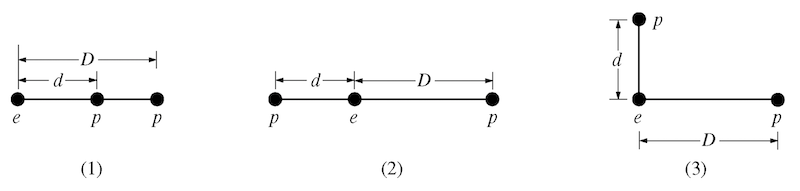
\includegraphics{./images/hw1/01-pgre.png}
\caption{particles}
\end{figure}

\begin{enumerate}
\def\labelenumi{\arabic{enumi}.}
\tightlist
\item
  The figure above shows three arrangements of one electron (\(e\)) and
  two protons (\(p\)). Which of the following is true about the
  magnitude \(F\) of the net electrostatic force acting on the electron
  due to the protons?
\end{enumerate}

\begin{itemize}
\tightlist
\item
  \(F_1 > F_2 > F_3\)
\item
  \(F_1 = F_2 > F_3\)
\item
  \(F_1 > F_3 > F_2\)
\item
  \(F_2 > F_1 > F_3\)
\item
  \(F_2 > F_3 > F_1\)
\end{itemize}

\begin{enumerate}
\def\labelenumi{\arabic{enumi}.}
\setcounter{enumi}{1}
\tightlist
\item
  Explain how you arrived at your answer. What physical principle(s) is
  this question testing your understanding of?
\end{enumerate}

\end{document}
